\documentclass[9pt]{beamer}
%\usefonttheme{serif} 
\usepackage{multimedia}
\usepackage[scaled=.90]{helvet}
\usepackage{courier}
\usepackage[T1]{fontenc}
\usepackage{graphicx}
\usepackage{amsmath}
\usepackage{caption}
\usepackage{tabularx}
%This is a semiar template 
%created by Bijumon T
%Asst.Prof. In Computer Engg:
%Model Engg: College

\usetheme{JuanLesPins}
\begin{document}
\begin{frame}
%\flushleft{}
\title {\textbf{File Sharing Application using P2P Protocol}\\
}
\author { Emmanuel Antony (22) \\
Malavika S Menon (32)\\
Rose Joseph (48) \\
Varun Krishna S (61)\\ 
\hfill \break
Govt. Model Engineering College\\
 Thrikkakkara }
\maketitle
\end{frame}

\begin{frame}[shrink]{Outline}
\tableofcontents
\end{frame}

\section{Introduction}
\begin {frame}[shrink]{Introduction}
\begin{itemize}
\item At present, no major app provides a smooth user experience for transferring files using peer-to-peer protocols. 
\item We intend to develop a web application, with enhanced user experience for easier transfer of files based on P2P protocol.
\item  This would also help enhance speed and divide the payload borne by the sender for sharing the file to a large number of users. 
\end{itemize}
\end{frame}

\section{Areas of Interest}
\begin{frame} {Areas of Interest}

\begin{itemize}
	 \item Computer Networks
     \item Web \& App Development
\end{itemize}
\end {frame}

\section{Existing Systems }
\begin{frame} {Existing Systems }
The primary modes of sharing files that can be compared with the proposed solution are based on
\begin{itemize}
    \item WiFi Direct (Xender/ShareIt)
    \item Messaging Application(Whatsapp/Telegram)
    \item Cloud (Google Drive/Dropbox)
\end{itemize}
\end{frame} 

\subsection{WiFi Direct - Xender/ShareIt}
\begin{frame}{WiFi Direct - Xender/ShareIt}
 \begin{itemize}
     \item These Apps work using a technology called WiFi direct. It uses the WiFi card in your phone to connect with another device. 
     \item It sets up a private connection between the two devices so that you will be able to transfer files without any interference at very high speeds. 
     \item It is very similar to Bluetooth, one device acts as a server while the other is the client. The first step is creating a connection between the sockets of the two devices. 
     \item Once these dynamic sockets are linked you will be able to send data between them both.
 \end{itemize}
 \end{frame}

\subsection{Messaging Application - Whatsapp/Telegram/Signal}
\begin{frame}{Messaging Application}
 \begin{itemize}
     \item Traditional messaging applications like WhatsApp, Telegram and Signal can be used to share files. These apps upload the files onto a common server and the clients in the group can redownload it anytime they want.
     \item They go for a server client model. Works really well when the server is up and online.
     \item If the server is offline, like the Facebook downtime recently, using these services to share files is near impossible
     \item The exact mechanism by which the file is transferred differs based on the application
 \end{itemize}
                 
\end{frame}


\subsection{Cloud - Google Drive/Dropbox}
\begin{frame}{Cloud - Google Drive/Dropbox}
 \begin{itemize}
     \item Sharing files using cloud is a quick and easy process.
     \item Centralised servers are usually fast and upload and download speeds are quick.
     \item Like messaging applications, there is a single point of failure. And if cloud service provider is unavailable or if there is a server downtime, then using these services becomes near impossible.
    %  \item Google is closed source so we wouldn’t know how the files are stored, unless we manually encrypt it and upload it. There are privacy concerns that lie with it. 
 \end{itemize}
\end{frame}

\section{Disadvantages of Existing System}
\begin{frame}{Disadvantages of Existing System}
 \begin{itemize}
     \item Wifi Direct limited by capability of mobile hotspot. Uses direct point to point communication. 
     \item Cloud - Bandwidth wastage, one central server whose downtime will affect the entire network. 
     \item Messaging Applications - Focuses on a different area of messaging with file sharing, where as our application prioritises file sharing. 
 \end{itemize}
\end{frame}

\section{Why P2P?}
\begin{frame}{Why P2P?}
 \begin{itemize}
     \item Peer-to-peer is a model in which everyone becomes a server. There is no central server; everyone who uses the network acts as their own server. \item Speed on a traditional web host is quite limited. Especially for larger files, it would require a burst of speed that isn't sustainable for long periods and locks the server up for other users. Bandwidth is also costly. 
     \item In the client-server model, performance degrades with more users, as the same amount of bandwidth is shared among more people.
     \item In P2P, it's actually faster when more users download a file. Instead of taking the whole file from one user, you're taking smaller pieces from hundreds or thousands of others. Even if they only have a little bandwidth to spare, the combined connections mean you get the maximum speed possible. 
 \end{itemize}
    
\end{frame}


\section{Proposed System - Features }
\begin{frame}{Proposed System - Features }
 \begin{itemize}
     \item To use the existing torrent protocol as the base layer protocol and solve UI/UX pain points with respect to torrenting a file. 
     \item Have groups to which files can be shared easily p2p via the application instead of having to upload the asset to a centralised server.
     \item The application is meant to be web based primarily (likely to be over UDP).
     \item Once this is accomplished, protocol layer innovations will also be considered to make p2p file sharing more efficient for specific niche use cases.
 \end{itemize}
\end{frame}

\section{Literature Survey}
\begin{frame}{}
    \large Literature Survey
\end{frame}
\begin{frame}{P2P Networking: An Information-Sharing Alternative}
Reference: 
\small M. Parameswaran, A. Susarla and A. B. Whinston, "P2P networking: an information sharing alternative," in Computer, vol. 34, no. 7, pp. 31-38, July 2001, doi: 10.1109/2.933501.
\break
\begin{itemize}
     \item This paper considers P2P networks as an alternative to traditional-client server models \& conveys the various advantages and disadvantages it offers. 
     \item A P2P network considers all nodes equal in their capacity for sharing information with other network members. 
     \item Each user makes an information repository available for distribution, which, combined with anyone’s ability to join the network, leads to the fast growth of a network composed of distributed information repositories
     \item Member nodes primarily use existing P2P networks, such as Gnutella or Napster, to share information of some kind. The TCP/IP Internet typically admits these nodes without restraint, and any node that can access the network can join.
\end{itemize}
\end{frame}
\begin{frame}{}
\begin{itemize}
    \item Individual nodes connecting to the network can access a real-time index of other active nodes and of the files they share. As soon as they connect, these nodes become part of the index themselves, with the files they choose to share automatically added to the index.
    \item Because the index provides addresses for resources available at any given time, a member node can simply initiate a direct connection with any connected member node that currently holds the requested information.
    \item Protocols for initiating such connections are part of P2P networks.
    \item Having a central node containing the full index can help with more efficient and faster search. However it is more susceptible to cause a network failure if the central node has some downtime. 
    \item P2P paradigm can be extended and enhanced to foster productivity in the workplace and support community activities.
\end{itemize}
    
\end{frame}
\begin{frame}{Searching}
    \begin{itemize}
        \item The search engines rely on Web crawlers that scour the Internet for content and store the information in massive, searchable databases. Such indexing only includes content from publicly operating servers, and the databases do not undergo immediate updates when any of those servers or links go down.
        \item In P2P, the information available at any user node is indexed, and remains indexed, only when the user is online.
        \item In a P2P network, search efficiency depends on how well organized the network is, its policies for classifying content and building directories, and the search software itself.
    \end{itemize}
     \begin{figure}
      \centering
      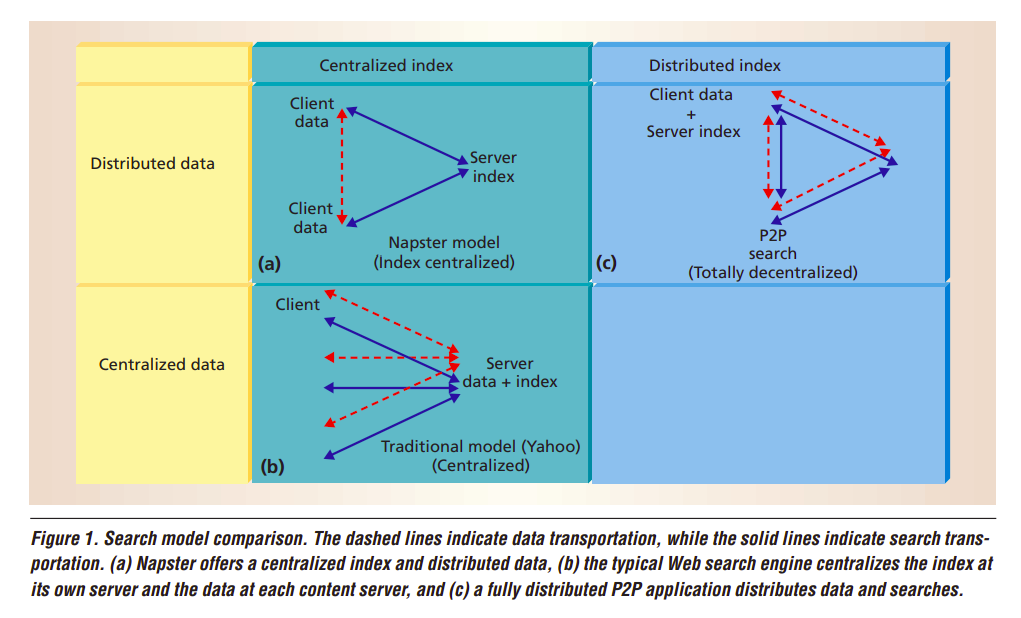
\includegraphics[width=7cm]{search.png}
  \end{figure}
\end{frame}
\begin{frame}{}
\begin{itemize}
    \item Disadvantages
\begin{itemize}
   \item P2P networks use protocols that allow individual nodes to participate easily, but this could result in decreased security. 
\item Without a central server, each node may only contain a partial index of the members it knows.This results in poorer efficiency for search and retrieval. 
\item Listed information may be cluttered with significant noise.
\item The Wild Web - Letting any user freely share any type of information raises issues of copyright infringement, intellectual piracy, and the potential spread of undesirable content.
\item There is the additional threat posed by crackers too, who may share malicious programs that could harm the individual user or result in denial of service attacks. 

\item But, under a controlled environment, P2P networks can be effective for sharing.
\end{itemize}
\end{itemize}
\end{frame}

\begin{frame}{}
\begin{itemize}
    \item Advantages

\begin{itemize}
    \item Enhanced load balancing:
Several techniques used to monitor traffic and redistribute content between nodes to ease the load on individual nodes and possibly locate content closer to points of high demand 
\item Dynamic Information Repository:
Any user can download information from a node and start distributing it too. So, content in high demand can be spread to other nodes. 
\item Redundancy and fault tolerance:
Replication of information at multiple nodes helps increase the availability. Decentralisation helps with fault tolerance. 
\item Content Based Addressing:
In P2P, the exact address of the node that stores a particular item remains transparent to the user.Addressing reaches a higher level in the semantic hierarchy because users specify a content identifier but not a physical location.
\end{itemize}
\end{itemize}
    
\end{frame}

\begin{frame}{PeerDB : A P2P-based System for Distributed Data Sharing}
\small {Reference: W. S. Ng, B. C. Ooi, K. -. Tan and Aoying Zhou, "PeerDB: a P2P-based system for distributed data sharing," Proceedings 19th International Conference on Data Engineering (Cat. No.03CH37405), 2003, pp. 633-644, doi: 10.1109/ICDE.2003.1260827.}
\break
\begin{itemize}
    \item This paper discusses the limitations of various P2P systems and how a distributed data sharing system like PeerDB(a prototype developed) will be useful. 
    \item Firstly, P2P systems offer only file level sharing and lack object/data management capabilities. 
    \item Second, they are limited in extensibility and flexibility.
    \item Third, a node's peers are typically statically defined. 
\end{itemize}
\end{frame}


\begin{frame}{Feature of PeerDB}
    \begin{itemize}
    \item Each participating node is a full-fledged object management system that supports content based search.
\item Users can share data without a global schema
\item Adopts mobile agents to assist in query processing. Since agents perform query processing in peer sites, network bandwidth is better utilised. 
\item Supports mechanisms to keep promising peers in close proximity based on some criterion.
\end{itemize}
\end{frame}

\begin{frame}{Architecture}
    \begin{itemize}
        \item The PeerDB application is built on top of  BestPeer.
        \item BestPeer is a generic P2P system. It consists of two entities - large number of computers and relatively fewer number of location independent global name lookup (LIGLO) servers.
        \item BestPeer integrates two powerful technologies - P2P and mobile agent. It shares not only data, but also computational power. 
        \item The architecture of a PeerDB node involves - Data Management System like MySQL, Database Agent system called DBAgent, cache manager and user interface. 
    \end{itemize}
\end{frame}

\begin{frame}{}
    \begin{figure}
      \centering
      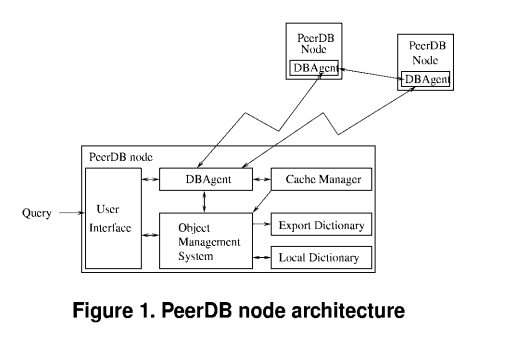
\includegraphics[width=7cm]{arch.png}
  \end{figure}
\end{frame}

\begin{frame}{}
\begin{itemize}
    \item Advantages
    \begin{itemize}
    \item Performs more than coarse level sharing of files
\item Better response time for queries 

\end{itemize}
\end{itemize}

\begin{itemize}
    \item Disadvantages
    \begin{itemize}
    \item Not primarily a file sharing application, mainly a distributed database management system.

\end{itemize}
\end{itemize}

\begin{itemize}
    \item Applications
    \begin{itemize}
    \item Health Care, Genomic Data, Data Caching

\end{itemize}
\end{itemize}
    
\end{frame}

\begin{frame}{The Bittorrent P2P File-Sharing System: Measurements and Analysis}
    \small Reference: THE BITTORRENT P2P FILE-SHARING SYSTEM: MEASUREMENTS AND ANALYSIS, J.A. Pouwelse, P. Garbacki, D.H.J. Epema, H.J. Sips, Department of Computer Science, Delft University of Technology, the Netherlands
    \break
    \begin{itemize}
        \item BitTorrent has attracted millions of users. Makes up around 53\% of all P2P traffic.
        \item Only a file-downloading protocol. In BitTorrent, files are split up into chunks, and the downloaders of a file barter for chunks of it by uploading and down-loading them in a tit-for-tat-like manner to prevent parasitic behavior. 
        \item It relies on other global components, such as web sites, for finding files. The most popular web site for this purpose was suprnova.org
    \end{itemize}
\end{frame}
\begin{frame}{}
\begin{itemize}    
    \item Advantages
        \begin{itemize}
            \item System of moderators help maintain the integrity of content on network and prevent pollution of data
\item Even average download speeds of 240 kbps allowed us to download large files in one day. 

        \end{itemize}
        \item Disadvantages
        \begin{itemize}
            \item Uses a global component like suprnova.org. When its server was down, it affected the entire network.
\item The system of moderators need global components, not distributed. 
\item When the popularity drops and the last peer/seed with certain content goes offline, the content dies. 
\item Peers should be given incentives to seed, such as bartering a file.

        \end{itemize}
    \end{itemize}
\end{frame}


\begin{frame}{Looking up data in P2P}
        \small Reference: Hari Balakrishnan, M. Frans Kaashoek, David Karger, Robert Morris, Ion Stoica
Communications of the ACM, February 2003, Vol. 46 No. 2, Pages 43-48
    \break
    \begin{itemize}
        \item The main challenge in P2P computing is to design and implement a robust and scalable distributed system composed of inexpensive, individually unreliable computers in unrelated administrative domains. The participants in a typical P2P system might include computers at homes, schools, and businesses, and can grow to several million concurrent participants.
        \item The ability to lookup data to access the data becomes very important in the process
        \item The paper disusses algorithms developed by several research groups for the lookup problem present a simple and general interface, a distributed hash table (DHT). Data items  are  inserted in  a  DHT  and found  by  specifying  a  unique  key
    \end{itemize}
\end{frame}
\begin{frame}{The Lookup Problem}
    \begin{itemize}
        \item The lookup problem is simple to state: Given a data item  X stored  at  some  dynamic  set  of  nodes  in  the system, find it. This problem is an important one in many  distributed  systems,  and  is  the  critical  common problem in P2P systems.
        \item The  traditional  approach  to  achieving  scalability
is  to  use  hierarchy.  The  Internet’s  Domain  Name System (DNS) does this for name lookups. Searches start  at  the  top  of  the  hierarchy  and,  by  following
forwarding references from node to node, traverse a single path down to the node containing the desired data. The disadvantage of this approach is that failure or removal of the root or a node sufficiently high in the hierarchy can be catastrophic, and the nodes higher  in  the  tree  take  a  larger  fraction  of  the  load than the leaf nodes.
    \end{itemize}
\end{frame}
\begin{frame}{Distributed Hash Table}
    \begin{itemize}
    \item A  hash-table  interface  is an  attractive  foundation for  a  distributed  lookup algorithm because it places  few  constraints  on the  structure  of  keys  or the values they name.The main requirements are that data be identified using unique numeric keys,  and  that  nodes be willing to store keys for each other. The values could be actual data items (file blocks), or could be pointers to where the data items are currently stored.
    \item A DHT implements just one operation:
lookup(key) yields  the  network  location  of  the
node currently responsible for the given key. A simple  distributed  storage  application  might  use  this interface as follows. To publish a file under a particular  unique  name,  the  publisher  would  convert  the name to a numeric key using an ordinary hash function  such  as  SHA-1,  then  call  lookup(key).  The publisher would then send the file to be stored at the node(s) responsible for the key. A consumer wishing to read that file would later obtain its name, convert it  to  a  key,  call  lookup(key),  and  ask  the  resulting
node for a copy of the file.
    \end{itemize}
\end{frame}
\begin{frame}
    \begin{itemize}
        \item Advantages
        \begin{itemize}
            \item Helps optimise the lookup problem in finding the location of the data
\item Does not require a centralised root server like the dns to enable the lookup 

        \end{itemize}
        \break
        \item Disadvantages
        \begin{itemize}
            \item All of the methods use a distributed hash table approach in discovering nodes
\item These algorithms retrieve data based on a unique identifier and keyword based search thereby making the user experience painful
        \end{itemize}
    \end{itemize}
\end{frame}


\begin{frame}{Multi-Torrent: a Performance Study}
     \small Reference: Y. Yang, A. L. H. Chow and L. Golubchik, "Multi-Torrent: a Performance Study," 2008 IEEE International Symposium on Modeling, Analysis and Simulation of Computers and Telecommunication Systems, 2008, pp. 1-8
    \break
    \begin{itemize}
        \item Incentivizing users to stay in a multi-torrent environment and investigates the performance impact due to the same 
        \item
            This paper gives the evidence for the fact that the existing bit torrent network lacks incentive for nodes to stay around as seeds in a multi-torrent environment
        \item It proposes cross torrent based strategy and then presents a simulation based performance study to illustrate the benefits
        \item Focuses on the questions:
           \begin{itemize}
               \item What incentives could be provided for nodes to contribute resources as seeds in a multi-torrent environment,
               \item What are the resulting performance consequences of such behavior, both on the nodes which are willing to be seeds and on the overall system.
           \end{itemize}
\end{itemize}
\end{frame}
\begin{frame}
    \begin{itemize}
\item Advantages
        \begin{itemize}
            \item Multiple torrents allows for faster download speeds
            \item Incentives are provided to the seeders so that they have reason to keep the torrent alive
        \end{itemize}
        \item Disadvantages
        \begin{itemize}
            \item The existing protocol has to be updated, and this might result in a loss of interoperability with other torrent clients
        \end{itemize}
    \end{itemize}
\end{frame}

\begin{frame}{Analyzing The DC File Sharing Network}
    \small Reference: P. Gurvich, N. Koenigstein and Y. Shavitt, "Analyzing the DC File Sharing Network," 2010 IEEE Tenth International Conference on Peer-to-Peer Computing (P2P), 2010, pp. 1-4
    \break
    \begin{itemize}
        \item The paper investigates the DC file sharing network.
        \item Direct Connect (DC) is a peer-to-peer file sharing protocol. Direct Connect clients connect to a central hub and can download files directly from one another.
        \item Hubs feature a list of clients or users connected to them. Users can search for files and download them from other clients, as well as chat with other users.
        \item DC was found to be the second most popular file sharing network in many places after BitTorrent.
        \item In this study they devised a participating agent for measuring and characterizing the DC file sharing network.
        \item This paper makes two main contributions:
             \begin{itemize}
                 \item It is the first measurement study of the DC network. 
                 \item While investigating this network we discovered a query duplication problem that stems the protocol’s scalability potential. Resolving this problem will reduce much of of the hubs CPU and bandwidth requirements and thus allow the hub communities to grow and accept more users.
             \end{itemize}
    \end{itemize}
\end{frame}
\begin{frame}{Analyzing The DC File Sharing Network - How it was done?}
    \begin{itemize}
        \item The DC network consists of regular users (clients) connected to one or more central hubs.
        \item Users manually choose hubs to connect to according to their area of interest or geographical location.
        \item Once a day, the agent downloads a DC hub list from a public hub-list server. It then initiate connection to the top 150 largest hubs. 
        \item The agent does not participate in the actual sharing activity. Instead it falsely reports its shared folder size and fakes its content. So some hubs reject and some hubs redirect to other hubs.
        \item Upon connection the agent records the hub’s user count and the total amount of shared content. 
        \item When a user joins or leaves the hub a \$MyINFO or \$Quit messages are sent by the hub to all users respectively. By monitoring these messages the agent can track the current number of connected users in a hub.
        \item The agent also monitors and records search queries received from the clients.
    \end{itemize}
\end{frame}
\begin{frame}{Analyzing The DC File Sharing Network - Observations}
\begin{itemize}
  \item Resolved the geographical location of peers in hubs using the IP address of their queries. While some of the big hubs have a wide diversity of users nationalities, many hubs are dominated by users from the same country.
  \item The number of users in a hub and its query frequency are highly correlated and reflect its activity.
  \item Text search queries reflect users taste and areas of interest. Recently, the content of P2P queries had been the focus of several studies in the field of data-mining and marketing.
  \hfill \break
  \begin{figure}
      \centering
      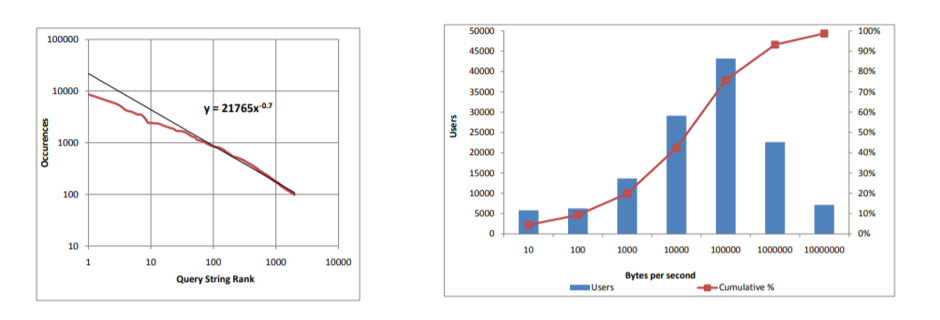
\includegraphics[width=7cm]{correlation_sharedData.png}
      \caption{a)Zipf law distribution of queries popularity;b)Change rate in active users shared folder}
      \label{}
  \end{figure}
\end{itemize}
\end{frame}
\begin{frame}{Analyzing The DC File Sharing Network - Observations}
    \begin{itemize}
       \item Ranked the top 10,000 most popular text queries collected during 4 days. It was suggested to take advantage of such a distribution by caching a small number of queries.
       \item Hub operators often set strict entry criteria to users, which is usually based on the amount of information a user shares. Although harsh to some users, this requirement reduces leeching effectively.
       \item The average shared folder size was 52.7 GB, which is considerably higher than users on other file sharing networks.
        \item Calculated the change in folder size between the first time a user was seen and the last time he/she was seen. Naturally, many users were idle and did not download any files and some users deleted content from their shared folder
        \item On average the active users monitored increased their shared folder by 74.7 KB per second, which means that at least 9.71 GB were swapped every second, or 3.36 PB over the entire period. 
    \end{itemize}
\end{frame}
\begin{frame}{Analyzing The DC File Sharing Network - The query duplication problem}
    \begin{itemize}
    \item The hubs most important role is to distribute queries to all connected peers. \item Clients with relevant content may answer directly to the searching peer, or use the hub as a proxy. Sharing is then performed in a pure P2P fashion. Hubs have no way of knowing which other hubs a user is connected to. 
    \item Inevitably users receive duplicated queries belonging to users with whom they share more than one hub. These redundant queries waste the hubs’ bandwidth and CPU resources eventually forcing the hub to reject incoming peers.
    \item On an average day, connected to approximately 122 hubs, we identified that about 40\% of the intercepted text queries were duplicated and only 60\% were original.
    \item They also measured the depth of the duplications for the ten largest hubs. The great majority of the duplicated queries (99.2\%) were seen on either 2 hubs (72.6\%) or on 3 hubs (26.6\%). Only a negligible fraction of the queries (0.8\%) were seen on more than 3 hubs.
    \end{itemize}
\end{frame}
\begin{frame}
\begin{itemize}
       \begin{figure}
           \centering
           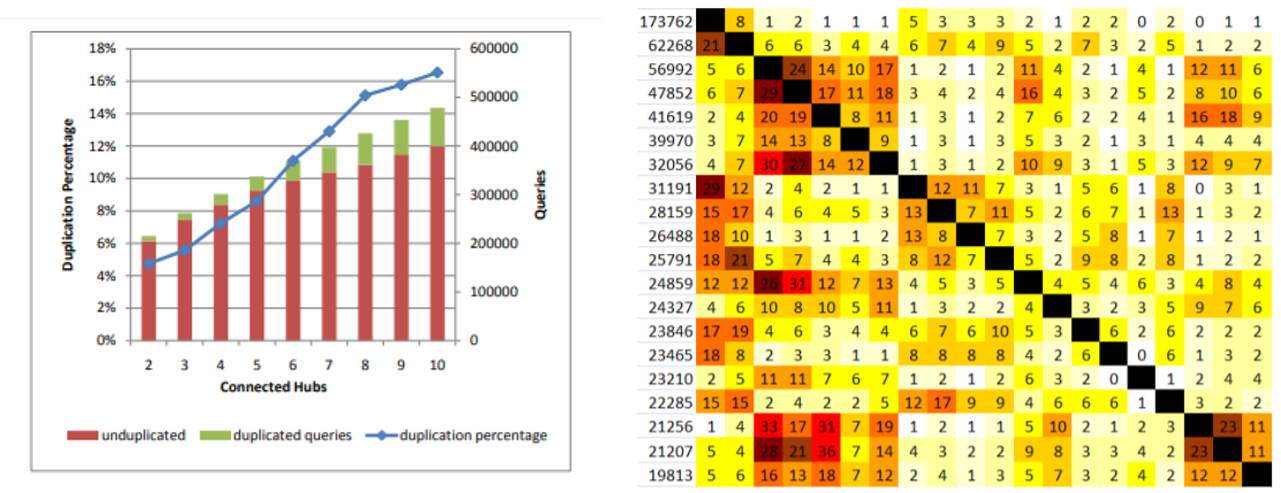
\includegraphics[width=8cm]{query_duplication.png}
           \caption{a)Percentage of duplicated queries per hubs
connected; b)Duplication Matrix}
           \label{fig:my_label}
       \end{figure}
        \item Advantages
        \begin{itemize}
            \item Users can select hubs which are geographically near, to get high speeds.
        \end{itemize}
        \item Disadvantages
        \begin{itemize}
            \item It doesn’t cache search queries.
            \item During a survey it was seen there was a lot of duplicate text queries (about 40\%)
        \end{itemize}
    \end{itemize}
\end{frame}

\begin{frame}{Comparison Table}
    \begin{tabularx}{1.0\textwidth} { 
        | >{\centering\arraybackslash}X
        | >{\centering\arraybackslash}X
        | >{\centering\arraybackslash}X
        | >{\centering\arraybackslash}X | }
        \hline Paper & Techniques & Pros & Cons \\
        \hline P2P Networking: An Information-Sharing Alternative & P2P network as a mode of file sharing over normal client/server model, no central server & Enhanced load balancing, redundancy and fault tolerance, content based addressing, dynamic information repository & Decreased security, copyright infringement, poorer search/retrieval time as nodes may contain only parietal information \\
        \hline PeerDB : A P2P-based System for Distributed Data Sharing & Participating node is a full fledged abject management system supporting content based search  & Good query response time, more fine than coarse file sharing & Not a file transferring applications primarily, works more as a distributed database \\
        \hline
    \end{tabularx}
\end{frame}

\begin{frame}{Comparison Table}
    \begin{tabularx}{1.0\textwidth} { 
        | >{\centering\arraybackslash}X
        | >{\centering\arraybackslash}X
        | >{\centering\arraybackslash}X
        | >{\centering\arraybackslash}X | }
        \hline Paper & Techniques & Pros & Cons \\
        \hline The BitTorrent P2P File-Sharing System: Measurements and Analysis & File downloading based on P2P network & Good average download speed of 240kbps and upwards, system moderators helps maintain integrity of the data & Peers should be incentivised, moderators need a global component not a distributed one, partial fault tolerance is non existent \\
        \hline Looking up data in P2P & Distributed hash table & Does not require a central server & Use a unique identifier and keyword search not supported \\
        \hline
    \end{tabularx}
\end{frame}

\begin{frame}{Comparison Table}
    \begin{tabularx}{1.0\textwidth} { 
        | >{\centering\arraybackslash}X
        | >{\centering\arraybackslash}X
        | >{\centering\arraybackslash}X
        | >{\centering\arraybackslash}X | }
        \hline Paper & Techniques & Pros & Cons \\
        \hline Multi-Torrent: a Performance Study & Multi Torrent seeding & Faster transfer speeds, incentivises users to seed & Slightly updated version of bit torrent protocol hence all clients may not support it \\
        \hline Analyzing The DC File Sharing Network & Hub model & Requires a central hub for distribution & Search queries are not cache, many duplicate text queries were present ``\\
        \hline
    \end{tabularx}
\end{frame}

\begin{frame}{Problem Statement}
    \begin{itemize}
        \item To develop a file sharing application using P2P which is robust, faster than traditional client-server models and with enhanced user experience.
    \end{itemize}
\end{frame}


\begin{frame}{Objectives}
   \begin{itemize}
       \item Torrent-based file sharing application for faster transfer of files simultaneously to multiple users.
       \item We intend to develop an Android application, with enhanced user experience for easier transfer of files based on P2P protocol.
       \item This would also help enhance speed and divide the payload borne by the sender for sharing the file to a large number of users.
       \item Instead of uploading the files to a centralised server, they can be shared to groups using p2p.
   \end{itemize}
    
\end{frame}

\begin{frame}{References}
    \begin{itemize}
        \item M. Parameswaran, A. Susarla and A. B. Whinston, "P2P networking: an informationsharing alternative," in Computer, vol. 34, no. 7, pp. 31-38, July 2001.
        \item W. S. Ng, B. C. Ooi, K. -. Tan and Aoying Zhou, "PeerDB: a P2P-based system fordistributed data sharing," Proceedings 19th International Conference on Data Engineering (Cat.No.03CH37405), 2003.
        \item THE BITTORRENT P2P FILE-SHARING SYSTEM: MEASUREMENTS ANDANALYSIS, J.A. Pouwelse, P. Garbacki, D.H.J. Epema, H.J. Sips, Department of ComputerScience, Delft University of Technology, the Netherlands
        \item Looking up data in P2P systems; Hari Balakrishnan, M. Frans Kaashoek, David Karger, Robert Morris, Ion StoicaCommunications of the ACM, February 2003, Vol. 46 No. 2, Pages 43-48.
        \item Y. Yang, A. L. H. Chow and L. Golubchik, "Multi-Torrent: a Performance Study," 2008IEEE International Symposium on Modeling, Analysis and Simulation of Computers andTelecommunication Systems, 2008. 
        \item P. Gurvich, N. Koenigstein and Y. Shavitt, "Analyzing the DC File Sharing Network,"2010 IEEE Tenth International Conference on Peer-to-Peer Computing (P2P), 2010.
    \end{itemize}
\end{frame}

\begin{frame}
 \large{ THANK YOU !!}
\end{frame}

\end{document}


\section{}
\begin{frame}
 \large {Thank You}
\end{frame}


\end{document}
